\section{Theoretical Background}
\subsection{Lattice}
A solid has typically a periodicity in the placing of its atoms. This property is called \emph{crystal structure}, which can be locally restricted due to occurring crystal defects. Exceptions are the amorphous solids, that behave like very viscous fluids and will not be treated here (see \cite{ashcroft, gerthsen}).\\
Bravais lattice\\
Points $\vec{R}$ with:
\begin{align}
	\vec{R} &= \sum_{i = 0}^{N_D} n_i \vec{a}_i
\end{align}
with linearly independent primitive vectors $\vec{a}_i$, $n_i \in \mathbb{Z}$ and the dimension $N_D$.\\

\emph{primitive (unit) cell}\\
Fills complete space without any overlap under all transitions $\vec{R}$\\

\emph{(conventional) unit cell}\\
Fills complete space without any overlap under a subset of transitions of $\vec{R}$. Sometimes preferred due to a different symmetry.\\

\emph{Wigner-Seitz primitive cell}\\
Primitive cell containing all space closer to a certain lattice point than to all others.\\


\emph{Reciprocal lattice}\\
Set of wave vectors $\vec{K}$, so that the plane wave has the periodicity of a given Bravais lattice:
\begin{align}
	\exp\left(i\vec{K}\cdot\vec{r}\right) &= \exp\left[i\vec{K}\cdot\left(\vec{r} + \vec{R}\right)\right] &\Leftrightarrow& &\vec{K}\cdot\vec{R} &= \mathbb{Z}\cdot 2\pi	
\end{align}
Therefore the wave vectors $\vec{K}$ form also a Bravais lattice called the \emph{reciprocal lattice}. The primitive vectors $\vec{b}_i$ of a three dimensional reciprocal lattice can be derived as follows:
\begin{align}
	\vec{b}_i = 2\pi \frac{\vec{a}_{i+1}\times\vec{a}_{i+2}}{\vec{a}_1 \cdot \left(\vec{a}_2 \times \vec{a}_3\right)}
\end{align}
where the indices have to be understood modulo 3.\\

\emph{First Brillouine Zone}\\
Wigner-Seitz cell of reciprocal lattice.\\

\subsection{Bloch Theorem}
According to Bloch's theorem a wave functions $\Psi(\vec{r})$ of a periodic potential, $V\big(\vec{r} + \vec{R}\big)= V\big(\vec{r}\big)$ for all $\vec{R}$ of a Bravais lattice, can be written in the form:

\begin{align}
	\Psi(\vec{r}) &= \exp\left(i\vec{k}\cdot\vec{r}\right) \cdot u\left(\vec{r}\right)
\end{align}
where $\vec{k}$ is an arbitrary wave vector and $u\left(\vec{r}\right)$ denotes a $\vec{R}$-periodic function.\\
Under the assumption, that the boundary condition at the surface should not change the physical properties of the bulk, one assumes the periodic \emph{Born-von Karman boundary condition}\footnote{Alternatively one can choose the boundary condition  for a vanishing wave function on the surface $\Psi\left(\vec{S}\right) = 0$. But the periodic boundary condition has the advantage, that it corresponds with propagating waves, which suite transport phenomena very well, whereas a vanishing boundary condition corresponds with standing waves.}:
\begin{align}
	\Psi\left(\vec{r} + N_i \vec{a}_i\right) &= \Psi\left(\vec{r}\right)
\end{align}
where $N_i$ denotes the number of unit cells in the direction $\vec{a}_i$ of the bulk. Hereby one obtains additional conditions for the wave vector $\vec{k}$, namely:
\begin{align}
	\vec{k} &= \sum_{i = 1}^{N_D} \frac{m_i}{N_i} \vec{b}_i & m_i \in \mathbb{Z} 
\end{align}
One considers that the number of states in the first Brillouine zone equals the number of sites $N = \prod_{i = 1}^{N_D}N_i$ of the bulk.\\

\newpage
\subsection{Polyacetylene Hamiltonian}
Hamiltonian for trans-polyacetylene:

\begin{figure}
	\centering
	\begin{tikzpicture}[show background rectangle, scale = 1]
		\pgfmathsetmacro{\j}{0.5};
		\draw (0,0) -- (6,0);
		\foreach \i in {0,2,...,6}{
			\draw[fill = black] ({\i + \j * (-1)^(\i/2)},0) circle (0.1);
			\draw[] (\i,-0.1) -- (\i, 0.1);
		}
		\draw[<->] (2 - \j, -1) -- (6 - \j, -1) node[midway, fill = white] {2a};
		\draw[<->] (0 + \j, -0.5) -- (4 + \j, -0.5) node[midway, fill = white] {2a};
		\draw[<->] (2 - \j, 0.5) -- (2, 0.5) node[midway, above] {$u$};
		\draw[<->] (4, 0.5) -- (4 + \j, 0.5) node[midway, above] {$u$};
		\draw[dotted] (-0.3,0) -- (6.3, 0);
	\end{tikzpicture}
	\caption{Schema: perfectly dimerized molecule}
	\label{image_schema_dimer}
\end{figure}
\begin{align}
	\mathcal{H} &= \underbrace{-2\sum_{n} t_{n+1,n}\left(c_{n+1}^\dagger c_n + c_n^\dagger c_{n+1}\right)}_{\text{electrone hopping}} +
	\underbrace{\frac{1}{2}\sum_n \kappa (u_{n+1} - u_n)^2}_{\sigma \text{ bonding energy}} + 
	\underbrace{\frac{1}{2} \sum_n M \dot{u}^2_n}_{\text{kinetic energy}}
\end{align}
Born-Oppenheimer and $u_n = (-1)^nu$, $\alpha = \nicefrac{\partial t}{\partial u}$, $\delta = 2\alpha u$ (see \cref{image_schema_dimer}):
\begin{align}
	\mathcal{H} &= -2\sum_n \left[t_0 + (-1)^n\delta\right]\cdot\left(c_{n+1}^\dagger c_n + c_n^\dagger c_{n+1}\right) + 2N\kappa u^2\\
	&= -2\sum_n^{N_d} \left[\left(t_0+\delta\right)\left(c_{2n+1}^\dagger c_{2n} + c_{2n}^\dagger c_{2n+1} \right) + 
	\left(t_0-\delta\right)\left(c_{2n}^\dagger c_{2n-1} + c_{2n-1}^\dagger c_{2n} \right)\right]+2N\kappa u^2\\
	&\neq -2\sum_n^{N_d} \left[\left(t_0+\delta\right)\left(c_{2n+1}^\dagger c_{2n} + c_{2n}^\dagger c_{2n+1} \right) + 
	\left(t_0-\delta\right)\left(\textcolor{red}{c_{2n+1}^\dagger c_{2n} + c_{2n}^\dagger c_{2n+1}}\right)\right]+2N\kappa u^2
\end{align}
Calculate creation and annihilation operator in k-space (symmetric normation factors):
\begin{align}
	c_{2n} &= \frac{1}{\sqrt{N_d}}\sum_k\exp\left[ik\left(2n\right)a\right]\cdot c_{k}^{(e)}\\
	c_{2n+1} &= \frac{1}{\sqrt{N_d}}\sum_k\exp\left[ik\left(2n+1\right)a\right]\cdot c_{k}^{(o)}\\
	c_k^{(e)} &= \frac{1}{\sqrt{N_d}}\sum_n \exp\left[-ik\left(2n\right)a\right]\cdot c_{2n}\\
	c_k^{(o)} &= \frac{1}{\sqrt{N_d}}\sum_n \exp\left[-ik\left(2n+1\right)a\right]\cdot c_{2n+1}
\end{align}
Remember: operators $c_{2n(+1)}$ operate on double unit cell length $\rightarrow$ halve Brillouin zone $\left(-\frac{\pi}{2a}, \frac{\pi}{2a}\right]$\\
boundary condition: $\exp\left[2ik\left(n+N_d\right)a\right] = 1 \rightarrow N_d$ allowed kpts in Brillouin zone\\
Check for $c_{2n}$:
\begin{align}
	c_{2n_0}(c_k^{(e)}(c_{2n_i})) &= c_{2n} \\
	&= \frac{1}{\sqrt{N_d}}\sum_k\exp\left[ik\left(2n_0\right)a\right]\cdot \frac{1}{\sqrt{N_d}}\sum_n \exp\left[-ik\left(2n\right)a\right]\cdot c_{2n}\\
	&= \frac{1}{N_d}\sum_{k, n} \exp\left[ika\left(2n_0-2n\right)\right]\cdot c_{2n}\\
	&= \frac{1}{N_d}\sum_n N_d \delta_{2n_0,2n} c_{2n}\\
	&= c_{2n_0}
\end{align}
Warm up calculation:
\begin{align}
	\sum_n^{N_d}c_{2n+1}^\dagger c_{2n} &=\sum_{n, k, k'} \exp\left[ika(2n)\right] \cdot \exp\left[-ik'a(2n+1)\right] \cdot \frac{c_{k'}^{\dagger(o)}c_k^{(e)}}{N_d} \\
	&=\sum_{n, k, k'} \exp\left[ia(k-k')(2n)\right] \cdot \exp\left(-ik'a\right) \cdot  \frac{c_{k'}^{\dagger(o)}c_k^{(e)}}{N_d} \\
	&=\sum_{k, k'} \delta_{k, k'} \cdot \exp\left(-ik'a\right)\cdot c_{k'}^{\dagger(o)}c_k^{(e)}\\
	&=\sum_{k'} \exp\left(-ik'a\right) \cdot c_{k'}^{\dagger(o)}c_{k'}^{(e)}
\end{align}
Analogously:
\begin{align}
	\sum_n^{N_d} c_{2n}^\dagger c_{2n+1} &=\sum_{k'} \exp\left(ik'a\right)\cdot c_{k'}^{\dagger(e)}c_{k'}^{(o)}\\
	\sum_n^{N_d} c_{2n}^\dagger c_{2n-1}&=\sum_{k'} \exp\left(-ik'a\right)\cdot  c_{k'}^{\dagger(e)}c_{k'}^{(o)}\\
	\sum_n^{N_d} c_{2n-1}^\dagger c_{2n} &=\sum_{k'} \exp\left(ik'a\right)\cdot  c_{k'}^{\dagger(o)}c_{k'}^{(e)}
\end{align}
Thus one obtains:
\begin{align}
	\mathcal{H} &= -2\sum_n^{N_d} \left[\left(t_0+\delta\right)\left(c_{2n+1}^\dagger c_{2n} + c_{2n}^\dagger c_{2n+1} \right) + 
	\left(t_0-\delta\right)\left(c_{2n+2}^\dagger c_{2n+1} + c_{2n+1}^\dagger c_{2n+2}\right)\right]+2N\kappa u^2\\
	&= -2\sum_{k'} \left[\left(t_0+\delta\right)\left(\exp\left(-ik'a\right) \cdot c_{k'}^{\dagger(o)}c_{k'}^{(e)} + \exp\left(ik'a\right)\cdot c_{k'}^{\dagger(e)}c_{k'}^{(o)}\right)+ \right.\nonumber\\
	&\hspace*{1.6cm}\left.\left(t_0-\delta\right)\left(\exp\left(-ik'a\right)\cdot  c_{k'}^{\dagger(e)}c_{k'}^{(o)}+\exp\left(ik'a\right)\cdot  c_{k'}^{\dagger(o)}c_{k'}^{(e)}\right)\right]+2N\kappa u^2\\
	&= -2\sum_{k'} \left\{\left[2t_0\cos(k'a) + 2i\delta\sin(k'a)\right]c_{k'}^{\dagger(e)}c_{k'}^{(o)} + \right.\nonumber\\
	&\hspace*{1.7cm}\left. \left[2t_0\cos(k'a)-2i\delta\sin(k'a)\right] c_{k'}^{\dagger(o)}c_{k'}^{(e)}\right\}+2N\kappa u^2\\
	&\neq-2\sum_{k'} \left\{\left[\textcolor{red}{-}2t_0\cos(k'a) + 2i\delta\sin(k'a)\right]c_{k'}^{\dagger(e)}c_{k'}^{(o)} + \right.\nonumber\\
	&\hspace*{1.7cm}\left. \left[\textcolor{red}{-}2t_0\cos(k'a)-2i\delta\sin(k'a)\right] c_{k'}^{\dagger(o)}c_{k'}^{(e)}\right\}+2N\kappa u^2
\end{align}
Substituting $\epsilon_k := 2t_0\cos(ka)$ and $\Delta_k := 2\delta\sin(ka)$ the following form of the hopping term can be derived:
\begin{align}
	\mathcal{H}_{\text{hopp},k} &=
	\left[\epsilon_k + i\Delta_k\right]c_{k}^{\dagger(e)}c_{k}^{(o)} + \left[\epsilon_k-i\Delta_k \right]	c_{k}^{\dagger(o)}c_{k}^{(e)}
\end{align}
with the eigenvalues $E_k = \pm \sqrt{\epsilon_k^2+\Delta_k^2}$ and the eigenfunctions
\begin{align}
	\Psi_k^{(c)} &= \frac{1}{\sqrt{2}}\left(c_k^{\dagger(e)}+\frac{\epsilon_k - i \Delta_k}{|E_k|}c_{k}^{\dagger(o)}\right)\\
	\Psi_k^{(v)} &= \frac{1}{\sqrt{2}}\left(c_k^{\dagger(e)}-\frac{\epsilon_k - i \Delta_k}{|E_k|}c_{k}^{\dagger(o)}\right)
\end{align}
corresponding to the valance $(v)$ and conduction $(c)$ band. Hereby the eigenfunctions have to be understood as operating on the vacuum state, $|(e),(o)\rangle = |0,0\rangle$. Due to this one can check the orthogonality and normalization, for example:
\begin{align}
\left\langle\Psi_k^{(v)}\Big|\Psi_k^{(v)}\right\rangle &= \frac{1}{2}
\left(c_k^{(e)}-\frac{\epsilon_k + i \Delta_k}{|E_k|}c_{k}^{(o)}\right)
\left(c_k^{\dagger(e)}-\frac{\epsilon_k - i \Delta_k}{|E_k|}c_{k}^{\dagger(o)}\right)\\
&= \frac{1}{2} \left[c_k^{(e)}c_k^{\dagger(e)}+\frac{\left(\epsilon_k-i\Delta_k\right)\left(\epsilon_k+i\Delta_k\right)}{\left|E_k\right|^2}c_k^{(o)}c_k^{\dagger(o)}\right.\nonumber\\
&\hspace*{1cm}\left.-\frac{\epsilon_k+i\Delta_k}{|E_k|}c_k^{(o)}c_k^{\dagger(e)}-\frac{\epsilon_k-i\Delta_k}{|E_k|}c_k^{(e)}c_k^{\dagger(o)}\right]\\
&= \frac{1}{2}\left[c_k^{(e)}c_k^{\dagger(e)}+c_k^{(o)}c_k^{\dagger(o)}\right]\\
&= 1
\end{align}
Check also the correspondence to the correct eigenvalues:
\begin{align}
	\left\langle\Psi_k^{(v)}\Big|\mathcal{H}_{\text{hopp},k}\Big|\Psi_k^{(v)}\right\rangle &=  \left[\frac{1}{\sqrt{2}}\left(c_k^{(e)}-\frac{\epsilon_k + i \Delta_k}{|E_k|}c_{k}^{(o)}\right)\right]\cdot\nonumber \\
	&\hspace*{.5cm}\left[
	\left[\epsilon_k + i\Delta_k\right]c_{k}^{\dagger(e)}c_{k}^{(o)} + \left[\epsilon_k-i\Delta_k \right]	c_{k}^{\dagger(o)}c_{k}^{(e)}
	\right]\cdot\nonumber\\
	&\hspace*{.5cm}\left[\frac{1}{\sqrt{2}}\left(c_k^{\dagger(e)}-\frac{\epsilon_k - i \Delta_k}{|E_k|}c_{k}^{\dagger(o)}\right)\right]\\
	&=  \frac{1}{2}\left[-\frac{(\epsilon_k-i\Delta_k)(\epsilon_k+i\Delta_k)}{|E_k|}-\frac{(\epsilon_k-i\Delta_k)(\epsilon_k+i\Delta_k)}{|E_k|}\right]\\
	&= - |E_k|\\
	\left\langle\Psi_k^{(c)}\Big|\mathcal{H}_{\text{hopp},k}\Big|\Psi_k^{(c)}\right\rangle &= |E_k|
\end{align}
Hence it is shown explicitly, that the energies of the valence band are decreased by $-|E_k|$ and the energies of the conduction band are increased by $|E_k|$. Using this the ground state energy can be derived as follows (completely occupied valence, empty conduction band):
\begin{align}
	E_0(u) &=-2\sum_k |E_k| + 2N\kappa u^2\\
	&= -2\sum_k \sqrt{\epsilon_k^2+\Delta_k^2} + 2N\kappa u^2\\
	&= -2\sum_k \sqrt{\left[2t_0\cos(ka)\right]^2+\left[2\delta\sin(ka)\right]^2} + 2N\kappa u^2\\
\end{align}
In the limit of $N \rightarrow \infty$ the sum becomes an integral:
\begin{align}
	E_0(u) &= \frac{-N}{\pi}\int\limits_{\nicefrac{-\pi}{2a}}^{\nicefrac{\pi}{2a}}\hspace*{-0.2cm}\text{d}k\ \sqrt{\left[2t_0\cos(ka)\right]^2+\left[2\delta\sin(ka)\right]^2} + 2N\kappa u^2\\
	&=\frac{-4Nt_0}{\pi}\underbrace{\int\limits_{0}^{\nicefrac{\pi}{2}}\text{d}\theta\ \sqrt{1-\left(1-\frac{\delta}{t_0}\right)\sin^2(\theta)}}_{=:I(\nicefrac{\delta}{t_0})} + 2N\kappa u^2
\end{align}
For small $\nicefrac{\delta}{t_0}$ the integral can be approximated as follows:
\begin{align}
	I\left(\frac{\delta}{t_0}\right) &\approx 1 + \frac{1}{2} \left[\ln\left(\frac{4|t_0|}{|\delta|}\right)-\frac{1}{2}\right]\frac{\delta^2}{t_0^2} 
\end{align}
To calculate the energies in manually charged states (cdft), use the states:
\begin{align}
		\Psi_k^{(v)}(q) &= \sqrt{\frac{1}{2}-\frac{q}{2}}c_k^{\dagger(e)}- \sqrt{\frac{1}{2}+\frac{q}{2}}\frac{\epsilon_k - i \Delta_k}{|E_k|}c_{k}^{\dagger(o)}
\end{align}
To test for the correct properties one calculates $\left|\left\langle c^{(*)}_k|\Psi_k^{(v)}(q)\right\rangle\right|^2$, for example:
\begin{align}
	\left|\left\langle c^{\dagger(e)}_k|\Psi_k^{(v)}(q)\right\rangle\right|^2 &= \left|c_k^{(e)} \left(\sqrt{\frac{1}{2}-\frac{q}{2}}c_k^{\dagger(e)}- \sqrt{\frac{1}{2}+\frac{q}{2}}\frac{\epsilon_k - i \Delta_k}{|E_k|}c_{k}^{\dagger(o)}\right)\right|^2\\
	&= \frac{1-q}{2}
\end{align}
Because of the two different spin orientations of the electron an additional factor 2 has to be taken into account to get the correct number of valence electrons at the even/odd positions. Therefore the number of valence electrons is given by $1 \pm q$. The energies for this states are given by:
\begin{align}
	\left\langle\Psi_k^{(v)}(q)\Big|\mathcal{H}_{\text{hopp},k}\Big|\Psi_k^{(v)}(q)\right\rangle &= \left[\sqrt{\frac{1-q}{2}}c_k^{(e)}- \sqrt{\frac{1+q}{2}}\frac{\epsilon_k + i \Delta_k}{|E_k|}c_{k}^{(o)}\right]\cdot\nonumber\\
	&\hspace*{0.5cm}\left[
	\left[\epsilon_k + i\Delta_k\right]c_{k}^{\dagger(e)}c_{k}^{(o)} + \left[\epsilon_k-i\Delta_k \right]	c_{k}^{\dagger(o)}c_{k}^{(e)}
	\right]\cdot\nonumber\\
	&\hspace*{0.5cm}\left[\sqrt{\frac{1-q}{2}}c_k^{\dagger(e)}- \sqrt{\frac{1+q}{2}}\frac{\epsilon_k - i \Delta_k}{|E_k|}c_{k}^{\dagger(o)}\right]\\
	&=-\sqrt{\frac{1-q}{2}}c_k^{(e)}\left[\epsilon_k+i\Delta_k \right]	c_{k}^{\dagger(e)}c_{k}^{(o)}\sqrt{\frac{1+q}{2}}\frac{\epsilon_k - i \Delta_k}{|E_k|}c_{k}^{\dagger(o)}\nonumber\\
	&\hspace*{0.4cm}-\sqrt{\frac{1+q}{2}}\frac{\epsilon_k + i \Delta_k}{|E_k|}c_{k}^{(o)}\left[\epsilon_k - i\Delta_k\right]c_{k}^{\dagger(o)}c_{k}^{(e)}\sqrt{\frac{1-q}{2}}c_k^{\dagger(e)}\\
	&=-\sqrt{\frac{1+q}{2}}\sqrt{\frac{1-q}{2}}\left[\frac{(\epsilon_k-i\Delta_k)(\epsilon_k+i\Delta_k)}{|E_k|}+\frac{(\epsilon_k-i\Delta_k)(\epsilon_k+i\Delta_k)}{|E_k|}\right]\\
	&= -\sqrt{1-q^2} |E_k|
\end{align}
For this reason the expected ground state energy  as a function of the transferred charge in respect of a negligible small  phonon coupling constant $\delta$ has the form:
\begin{align}
	E_0(q, u) &= -\frac{4Nt_0}{\pi} \sqrt{1-q^2} + 2N\kappa u^2
\end{align}  
Fit this function with simulation results for small q, see \cref{image_cdft_many_kpts}. Optimized fit coefficient:
\begin{align}
	t_0 &= \unit[9,4]{eV}\qquad\text{from fit}\\
	t_0 &= \unit[2.5]{eV}\qquad\text{Glen paper}
\end{align}
\begin{figure}
\centering
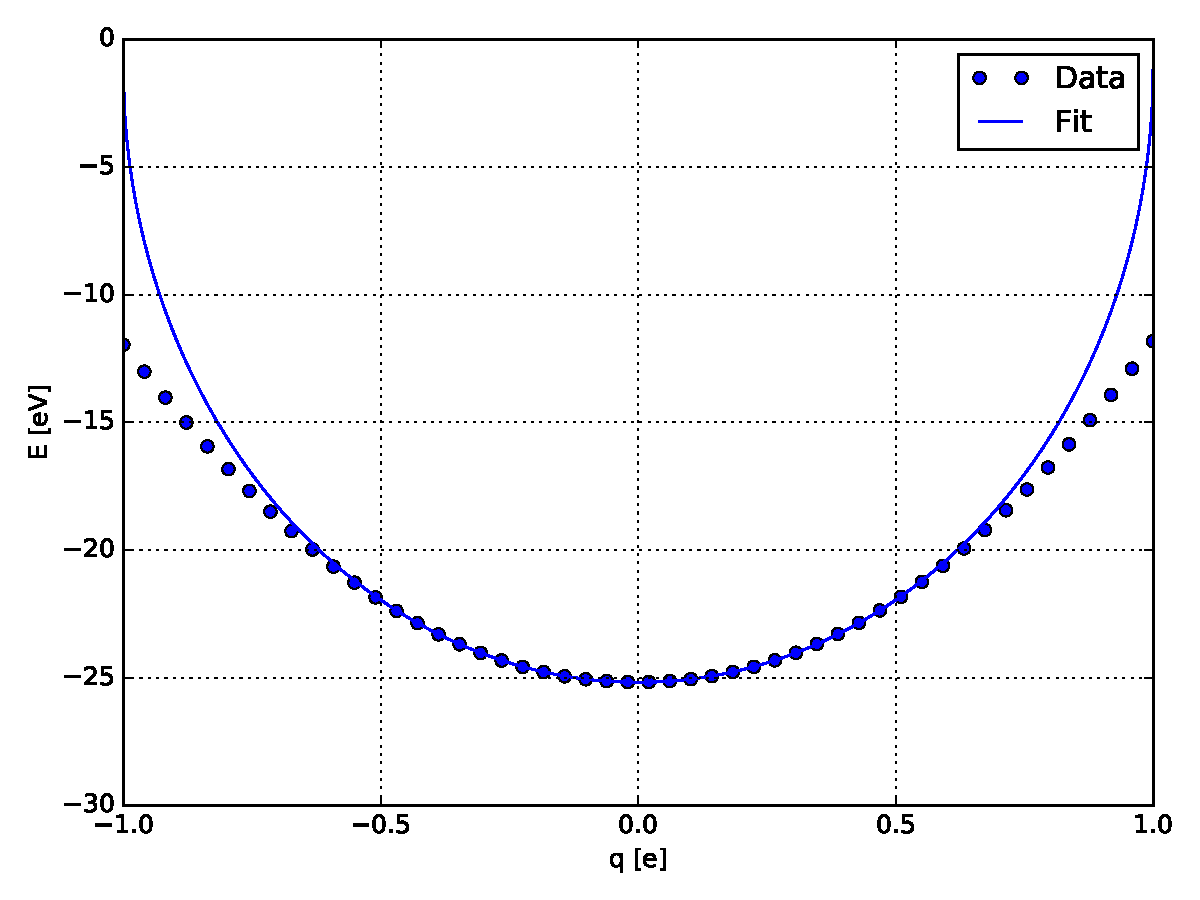
\includegraphics[width = \textwidth]{Images/CDFT/cdft_energy_many_kpts.pdf}
\caption[Unit cell energy as function of the manually shiftet charge for many k-points]{Unit cell energy as function of the manually shiftet charge for many k-points}
\label{image_cdft_many_kpts}
\end{figure}
Probably this assumption is wrong:
\begin{align}
	\Psi_k^{(v)}(q) &= \sqrt{\frac{1-q}{2}}c_k^{\dagger(e)}- \sqrt{\frac{1+q}{2}}\frac{\epsilon_k - i \Delta_k}{|E_k|}c_{k}^{\dagger(o)}
\end{align}
and should rather be formulated in a more general way:
\begin{alignat}{3}
	&&\Psi_k^{(v)}(q_k) &= \sqrt{\frac{1-q_k}{2}}c_k^{\dagger(e)}- \sqrt{\frac{1+q_k}{2}}\frac{\epsilon_k - i \Delta_k}{|E_k|}c_{k}^{\dagger(o)}\\
\Rightarrow&\qquad&\left\langle\Psi_k^{(v)}(q_k)\Big|\mathcal{H}_{\text{hopp},k}\Big|\Psi_k^{(v)}(q_k)\right\rangle &= -\sqrt{1-q^2_k} |E_k|
\end{alignat}
\newpage

\section{Other Preparations}
\begin{figure}
\centering

\begin{tikzpicture}[show background rectangle, scale = 1]
\foreach \x in {0,...,7}{
	\draw[line width=2pt] (\x,0) .. controls (\x + 1, 2) and (\x - 1 , 2) .. cycle .. controls (\x + 1, -2) and (\x - 1 , -2) .. cycle;
}
\foreach \x in {0, 4}
	\foreach \y in {0, 1}
		\foreach \z in {-1, 1}
		\node at (\x + \y - \z + 1, \z) {\huge +};
\foreach \x in {0, 4}{
	\foreach \y in {0, 1}{
		\foreach \z in {-1, 1}{
			\node at (\x + \y - \z + 1, -\z) {\huge -};
}}}
\draw[line width = 0.2] (-0.1, -1.8) -- +(-0.3, 0) -- +(-0.3 ,3.6) -- +(0,3.6);
\draw[line width = 0.2] (1.1, -1.8) -- +(0.3, 0) -- +(0.3 ,3.6) -- +(0,3.6);
\draw[line width = 0.2] (3.9, -1.8) -- +(-0.3, 0) -- +(-0.3 ,3.6) -- +(0,3.6);
\draw[line width = 0.2] (7.1, -1.8) -- +(0.3, 0) -- +(0.3 ,3.6) -- +(0,3.6);
\end{tikzpicture}
\end{figure}